% notes.tex


See \cite{AbbottUnderstandingAnalysis} for an intuition-driven introduction
to upper and lower bounds and the least upper bound property.











\subsection{Field Axioms of the Real Numbers}

The real numbers $\mathbb{R}$ form a \emph{field}. This means that $\mathbb{R}$ is a set
equipped with two binary operations, addition $(+)$ and multiplication $(\cdot)$,
satisfying the following axioms.

\subsubsection*{Additive Axioms}

\begin{description}

\item[\textbf{Axiom A1 (Additive Closure).}]
For all $x,y \in \mathbb{R}$, the sum $x+y \in \mathbb{R}$.

\[
\forall x \forall y \, (x,y \in \mathbb{R} \rightarrow x+y \in \mathbb{R})
\]

\item[\textbf{Axiom A2 (Additive Commutativity).}]
For all $x,y \in \mathbb{R}$,
\[
x+y = y+x.
\]

\[
\forall x \forall y \, (x+y = y+x)
\]

\item[\textbf{Axiom A3 (Additive Associativity).}]
For all $x,y,z \in \mathbb{R}$,
\[
(x+y)+z = x+(y+z).
\]

\[
\forall x \forall y \forall z \, ((x+y)+z = x+(y+z))
\]

\item[\textbf{Axiom A4 (Additive Identity).}]
There exists an element $0 \in \mathbb{R}$ such that for all $x \in \mathbb{R}$,
\[
x+0 = x.
\]

\[
\exists 0 \, \forall x \, (x+0 = x)
\]

\item[\textbf{Axiom A5 (Additive Inverse).}]
For every $x \in \mathbb{R}$, there exists an element $-x \in \mathbb{R}$ such that
\[
x+(-x) = 0.
\]

\[
\forall x \, \exists y \, (x+y = 0)
\]

\end{description}

\subsubsection*{Multiplicative Axioms}

\begin{description}

\item[\textbf{Axiom M1 (Multiplicative Closure).}]
For all $x,y \in \mathbb{R}$, the product $x\cdot y \in \mathbb{R}$.

\[
\forall x \forall y \, (x,y \in \mathbb{R} \rightarrow x\cdot y \in \mathbb{R})
\]

\item[\textbf{Axiom M2 (Multiplicative Commutativity).}]
For all $x,y \in \mathbb{R}$,
\[
x\cdot y = y\cdot x.
\]

\[
\forall x \forall y \, (x\cdot y = y\cdot x)
\]

\item[\textbf{Axiom M3 (Multiplicative Associativity).}]
For all $x,y,z \in \mathbb{R}$,
\[
(x\cdot y)\cdot z = x\cdot (y\cdot z).
\]

\[
\forall x \forall y \forall z \, ((x\cdot y)\cdot z = x\cdot (y\cdot z))
\]

\item[\textbf{Axiom M4 (Multiplicative Identity).}]
There exists an element $1 \in \mathbb{R}$, with $1 \neq 0$, such that for all $x \in \mathbb{R}$,
\[
x\cdot 1 = x.
\]

\[
\exists 1 \, (1 \neq 0 \wedge \forall x \, (x\cdot 1 = x))
\]

\item[\textbf{Axiom M5 (Multiplicative Inverse).}]
For every $x \in \mathbb{R}$ with $x \neq 0$, there exists an element $x^{-1} \in \mathbb{R}$ such that
\[
x\cdot x^{-1} = 1.
\]

\[
\forall x \, (x \neq 0 \rightarrow \exists y \, (x\cdot y = 1))
\]

\end{description}

\subsubsection*{Distributive Axiom}

\begin{description}

\item[\textbf{Axiom D (Distributivity).}]
For all $x,y,z \in \mathbb{R}$,
\[
x\cdot (y+z) = x\cdot y + x\cdot z.
\]

\[
\forall x \forall y \forall z \, (x\cdot (y+z) = x\cdot y + x\cdot z)
\]

\end{description}

\subsubsection*{Remark}

The axioms above define the algebraic structure of a field. To characterize
$\mathbb{R}$ uniquely among fields, these axioms must be supplemented by:
\begin{itemize}
\item an \emph{order structure} (ordered field axioms), and
\item the \emph{completeness axiom}.
\end{itemize}



\subsection{Order Axioms of the Real Numbers}

The real numbers $\mathbb{R}$ form a \emph{totally ordered field}.
The order structure is given by a binary relation $\leq$ on $\mathbb{R}$
satisfying the following axioms.

\subsubsection*{Basic Order Axioms}

\begin{description}

\item[\textbf{Axiom O1 (Reflexivity).}]
Every real number is comparable to itself:
\[
x \le x \quad \text{for all } x \in \mathbb{R}.
\]

\[
\forall x \, (x \le x)
\]

\item[\textbf{Axiom O2 (Antisymmetry).}]
If two real numbers are mutually less than or equal, then they are equal:
\[
x \le y \text{ and } y \le x \implies x = y.
\]

\[
\forall x \forall y \, ((x \le y \wedge y \le x) \rightarrow x = y)
\]

\item[\textbf{Axiom O3 (Transitivity).}]
The order relation is transitive:
\[
x \le y \text{ and } y \le z \implies x \le z.
\]

\[
\forall x \forall y \forall z \, ((x \le y \wedge y \le z) \rightarrow x \le z)
\]

\item[\textbf{Axiom O4 (Totality / Trichotomy).}]
Any two real numbers are comparable:
\[
\text{for all } x,y \in \mathbb{R}, \quad x \le y \text{ or } y \le x.
\]

\[
\forall x \forall y \, (x \le y \vee y \le x)
\]

\end{description}

\subsubsection*{Order Compatibility with Addition}

\begin{description}

\item[\textbf{Axiom O5 (Order Preservation under Addition).}]
For all $x,y,z \in \mathbb{R}$,
\[
x \le y \implies x+z \le y+z.
\]

\[
\forall x \forall y \forall z \, (x \le y \rightarrow x+z \le y+z)
\]

\end{description}

\subsubsection*{Order Compatibility with Multiplication}

\begin{description}

\item[\textbf{Axiom O6 (Order Preservation under Positive Multiplication).}]
For all $x,y,z \in \mathbb{R}$ with $z \ge 0$,
\[
x \le y \implies xz \le yz.
\]

\[
\forall x \forall y \forall z \, ((x \le y \wedge 0 \le z) \rightarrow xz \le yz)
\]

\item[\textbf{Axiom O7 (Order Reversal under Negative Multiplication).}]
For all $x,y,z \in \mathbb{R}$ with $z \le 0$,
\[
x \le y \implies yz \le xz.
\]

\[
\forall x \forall y \forall z \, ((x \le y \wedge z \le 0) \rightarrow yz \le xz)
\]

\end{description}

\subsubsection*{Positivity Axiom}

\begin{description}

\item[\textbf{Axiom O8 (Existence of Positive Elements).}]
There exists a real number that is strictly greater than zero.

\[
\exists x \, (0 < x)
\]

\end{description}

\subsubsection*{Remark}

The axioms above define a \emph{total order} on $\mathbb{R}$ that is compatible
with the field operations. Together with the field axioms, they define an
\emph{ordered field}. To characterize $\mathbb{R}$ uniquely, one must further
assume the \emph{completeness axiom}.


\subsection{Intervals in the Real Numbers}

Intervals are fundamental subsets of the real line defined using the order
relation on $\mathbb{R}$. Let $a,b \in \mathbb{R}$ with $a < b$.

\subsubsection*{Bounded Intervals}

\begin{definition}[Open Interval]
The \emph{open interval} from $a$ to $b$ is the set
\[
(a,b) := \{ x \in \mathbb{R} : a < x < b \}.
\]

\[
\forall x \, (x \in (a,b) \leftrightarrow a < x \wedge x < b)
\]
\end{definition}

\begin{definition}[Closed Interval]
The \emph{closed interval} from $a$ to $b$ is the set
\[
[a,b] := \{ x \in \mathbb{R} : a \le x \le b \}.
\]

\[
\forall x \, (x \in [a,b] \leftrightarrow a \le x \wedge x \le b)
\]
\end{definition}

\begin{definition}[Half-Open Intervals]
The \emph{left-closed, right-open interval} is
\[
[a,b) := \{ x \in \mathbb{R} : a \le x < b \}.
\]

The \emph{left-open, right-closed interval} is
\[
(a,b] := \{ x \in \mathbb{R} : a < x \le b \}.
\]
\end{definition}

---

\subsubsection*{Unbounded Intervals}

\begin{definition}[Open Rays]
The \emph{open rays} determined by $a \in \mathbb{R}$ are
\[
(a,\infty) := \{ x \in \mathbb{R} : x > a \},
\qquad
(-\infty,a) := \{ x \in \mathbb{R} : x < a \}.
\]
\end{definition}

\begin{definition}[Closed Rays]
The \emph{closed rays} determined by $a \in \mathbb{R}$ are
\[
[a,\infty) := \{ x \in \mathbb{R} : x \ge a \},
\qquad
(-\infty,a] := \{ x \in \mathbb{R} : x \le a \}.
\]
\end{definition}

---

\subsubsection*{Degenerate and Trivial Intervals}

\begin{definition}[Degenerate Interval]
If $a=b$, the closed interval
\[
[a,a] = \{a\}
\]
is called a \emph{degenerate interval}.
\end{definition}

\begin{definition}[Empty Interval]
If $a>b$, the set
\[
(a,b) = \varnothing
\]
is called an \emph{empty interval}.
\end{definition}


\begin{remark}
Intervals are precisely the subsets of $\mathbb{R}$ with the property that if
$x<y<z$ and $x,z$ belong to the set, then $y$ also belongs to the set.
\end{remark}























 





\begin{figure}[h]
\centering
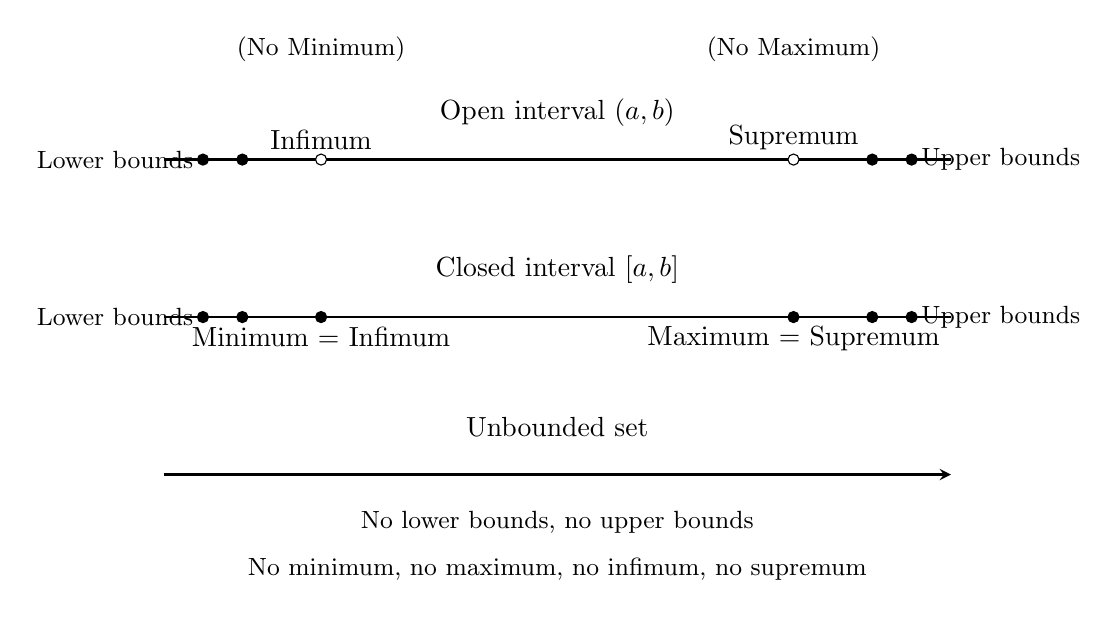
\begin{tikzpicture}[x=1cm,y=1cm,>=stealth]

% =====================
% OPEN INTERVAL (a,b)
% =====================
\draw[thick] (-5,3) -- (5,3);
\draw[fill=white] (-3,3) circle (2pt);
\draw[fill=white] (3,3) circle (2pt);

\node at (0,3.6) {Open interval $(a,b)$};

% Infimum / Supremum
\node[above] at (-3,3) {Infimum};
\node[above] at (3,3) {Supremum};
\node at (-3,4.4) {\small (No Minimum)};
\node at (3,4.4) {\small (No Maximum)};

% Lower bounds
\draw[fill] (-4.5,3) circle (2pt);
\draw[fill] (-4,3) circle (2pt);
\node[left] at (-4.5,3) {\small Lower bounds};

% Upper bounds
\draw[fill] (4,3) circle (2pt);
\draw[fill] (4.5,3) circle (2pt);
\node[right] at (4.5,3) {\small Upper bounds};

% =====================
% CLOSED INTERVAL [a,b]
% =====================
\draw[thick] (-5,1) -- (5,1);
\draw[fill] (-3,1) circle (2pt);
\draw[fill] (3,1) circle (2pt);

\node at (0,1.6) {Closed interval $[a,b]$};

% Min / Max
\node[below] at (-3,1) {Minimum = Infimum};
\node[below] at (3,1) {Maximum = Supremum};

% Lower bounds
\draw[fill] (-4.5,1) circle (2pt);
\draw[fill] (-4,1) circle (2pt);
\node[left] at (-4.5,1) {\small Lower bounds};

% Upper bounds
\draw[fill] (4,1) circle (2pt);
\draw[fill] (4.5,1) circle (2pt);
\node[right] at (4.5,1) {\small Upper bounds};

% =====================
% UNBOUNDED SET
% =====================
\draw[thick,->] (-5,-1) -- (5,-1);

\node at (0,-0.4) {Unbounded set};

\node at (0,-1.6)
{\small No lower bounds, no upper bounds};

\node at (0,-2.2)
{\small No minimum, no maximum, no infimum, no supremum};

\end{tikzpicture}
\caption{Bounds, extrema, infimum, and supremum for subsets of $\mathbb{R}$.}
\end{figure}



\begin{center}
\begin{tabular}{|p{4cm}|p{9cm}|}
\hline
\textbf{Concept} & \textbf{What you must show} \\
\hline

Upper bound &
To show that $u$ is an upper bound for $A$, prove that
\[
\forall a \in A,\quad a \le u.
\]
\\ \hline

Supremum &
To show that $u=\sup A$, prove:
\begin{itemize}
\item $u$ is an upper bound for $A$, and
\item every upper bound $v$ of $A$ satisfies $u \le v$.
\end{itemize}
\\ \hline

Bounded above &
To show that $A$ is bounded above, prove that
there exists at least one upper bound for $A$.
\\ \hline

Maximum &
To show that $m=\max A$, prove that $m$ is an upper bound for $A$
and that $m \in A$.
\\ \hline

\end{tabular}
\end{center}

% =========================================================
% Bounds, Suprema, and Infima — Formal Definitions
% =========================================================

\subsection{Bounds and Extremal Values}

\begin{definition}[Upper Bound]
Let $A \subseteq \mathbb{R}$.  
A number $u \in \mathbb{R}$ is an \emph{upper bound} for $A$ if
\[
\forall a \in A,\quad a \le u.
\]
\end{definition}

\begin{definition}[Lower Bound]
Let $A \subseteq \mathbb{R}$.  
A number $\ell \in \mathbb{R}$ is a \emph{lower bound} for $A$ if
\[
\forall a \in A,\quad \ell \le a.
\]
\end{definition}

\begin{definition}[Bounded Above / Below]
A set $A \subseteq \mathbb{R}$ is said to be:
\begin{itemize}
\item \emph{bounded above} if it has at least one upper bound;
\item \emph{bounded below} if it has at least one lower bound;
\item \emph{bounded} if it is both bounded above and bounded below.
\end{itemize}
\end{definition}

\begin{definition}[Supremum (Least Upper Bound)]
Let $A \subseteq \mathbb{R}$ be nonempty and bounded above.  
A number $s \in \mathbb{R}$ is the \emph{supremum} of $A$, written $s=\sup A$, if:
\begin{enumerate}
\item $s$ is an upper bound for $A$, and
\item if $u$ is any upper bound for $A$, then $s \le u$.
\end{enumerate}
\end{definition}

\begin{definition}[Infimum (Greatest Lower Bound)]
Let $A \subseteq \mathbb{R}$ be nonempty and bounded below.  
A number $i \in \mathbb{R}$ is the \emph{infimum} of $A$, written $i=\inf A$, if:
\begin{enumerate}
\item $i$ is a lower bound for $A$, and
\item if $\ell$ is any lower bound for $A$, then $\ell \le i$.
\end{enumerate}
\end{definition}

\begin{definition}[Maximum]
Let $A \subseteq \mathbb{R}$.  
A number $m \in A$ is a \emph{maximum} of $A$, written $m=\max A$, if
\[
\forall a \in A,\quad a \le m.
\]
\end{definition}

\begin{definition}[Minimum]
Let $A \subseteq \mathbb{R}$.  
A number $m \in A$ is a \emph{minimum} of $A$, written $m=\min A$, if
\[
\forall a \in A,\quad m \le a.
\]
\end{definition}

\subsection{Epsilon Characterizations}

\begin{definition}[Supremum — $\varepsilon$ Definition]
Let $A \subseteq \mathbb{R}$ be nonempty and bounded above, and let $s \in \mathbb{R}$.  
Then $s = \sup A$ if and only if:
\begin{enumerate}
\item $s$ is an upper bound for $A$, and
\item for every $\varepsilon > 0$, there exists $a \in A$ such that
\[
s - \varepsilon < a.
\]
\end{enumerate}
\end{definition}

\begin{definition}[Infimum — $\varepsilon$ Definition]
Let $A \subseteq \mathbb{R}$ be nonempty and bounded below, and let $i \in \mathbb{R}$.  
Then $i = \inf A$ if and only if:
\begin{enumerate}
\item $i$ is a lower bound for $A$, and
\item for every $\varepsilon > 0$, there exists $a \in A$ such that
\[
a < i + \varepsilon.
\]
\end{enumerate}
\end{definition}

\subsection{Directional $\varepsilon$-Characterizations}

\paragraph{Supremum: $\varepsilon$-approximation from below}

If $s=\sup A$, then:
\begin{itemize}
\item $s$ is an upper bound for $A$ (no element of $A$ exceeds $s$), and
\item no matter how close one approaches $s$ from below, there exist elements of $A$ arbitrarily close to $s$.
\end{itemize}

Equivalently,
\[
\forall \varepsilon>0,\ \exists a\in A \text{ such that } s-\varepsilon < a \le s.
\]

\paragraph{Infimum: $\varepsilon$-approximation from above}

If $i=\inf A$, then:
\begin{itemize}
\item $i$ is a lower bound for $A$ (no element of $A$ lies below $i$), and
\item no matter how close one approaches $i$ from above, there exist elements of $A$ arbitrarily close to $i$.
\end{itemize}

Equivalently,
\[
\forall \varepsilon>0,\ \exists a\in A \text{ such that } i \le a < i+\varepsilon.
\]









See \cite{RossElementaryAnalysis} for a clean axiomatic development of
bounds, suprema, and infima within ordered fields.

See \cite{BrucknerRealAnalysis} for a technically precise treatment of
bounds and extrema, including early exposure to subtle and pathological
examples.

See \cite{KolmogorovFominIntroAnalysis} for a classical, structurally
oriented approach to bounds and completeness with minimal pedagogical
scaffolding.

See \cite{LeblBasicAnalysisI} for a modern exposition of bounds and the
least upper bound property, accompanied by an extensive and well-curated
problem set.
